\documentclass{standalone}

\usepackage{tikz}
\usetikzlibrary{calc}

\begin{document}

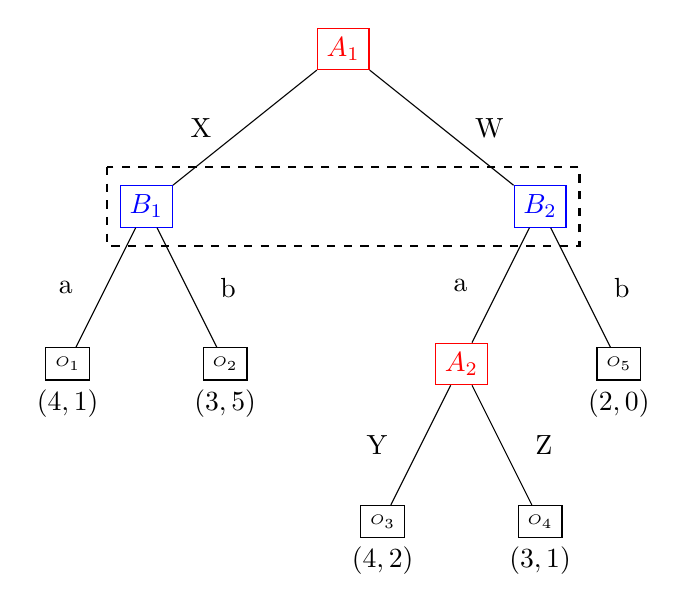
\begin{tikzpicture}
    \node [draw, color=red] (A1) at (0, 0) {\(A_1\)};
        \node [draw, color=blue] (B1) at ($(A1) + (-2.5, -2)$) {\(B_1\)};
            \node [draw] (O1) at ($(B1) + (-1, -2)$) {\tiny{\(O_1\)}};
            \node (SS) at ($(O1) + (0, -.5)$) {\((4, 1)\)};
            \node [draw] (O2) at ($(B1) + (1, -2)$) {\tiny{\(O_2\)}};
            \node (SC) at ($(O2) + (0, -.5)$) {\((3, 5)\)};
        \node [draw, color=blue] (B2) at ($(A1) + (2.5, -2)$) {\(B_2\)};
            \node [draw, color=red] (A2) at ($(B2) + (-1, -2)$) {\(A_2\)};
                \node [draw] (O3) at ($(A2) + (-1, -2)$) {\tiny{\(O_3\)}};
                \node (CS) at ($(O3) + (0, -.5)$) {\((4, 2)\)};
                \node [draw] (O4) at ($(A2) + (1, -2)$) {\tiny{\(O_4\)}};
                \node (CS) at ($(O4) + (0, -.5)$) {\((3, 1)\)};
            \node [draw] (O5) at ($(B2) + (1, -2)$) {\tiny{\(O_5\)}};
            \node (CC) at ($(O5) + (0, -.5)$) {\((2, 0)\)};

    \draw (A1) -- node[left=3mm] {X} (B1);
    \draw (A1) -- node[right=3mm] {W} (B2);
        \draw (B1)  -- node[left=3mm] {a} (O1);
        \draw (B1) -- node[right=3mm] {b} (O2);
        \draw (B2) -- node[left=3mm] {a} (A2);
            \draw (A2) -- node[left=3mm] {Y} (O3);
            \draw (A2) -- node[right=3mm] {Z} (O4);
        \draw (B2) -- node[right=3mm] {b} (O5);

    \draw  [dashed, thick] ($(B1) + (-.5, .5)$) rectangle  ($(B2) + (.5, -.5)$);
\end{tikzpicture}

\end{document}
